\patternFive

\subsection*{Context}

Graphics are an important way of presenting information for sighted people.  
Images are frequently used in electronic media such as websites and online platforms. In teaching, images are often used in web-based materials to convey content. Other digital resources - such as lecture notes, exercise sheets and presentation slides - also tend to contain a variety of images, graphics and illustrations.
    
\subsection*{Problem}

\begin{itshape}
Although electronic media can be made accessible to blind and visually impaired users through the use of assistive technologies, this does not usually work for the graphic components embedded in these media. As a result, the information conveyed by visual representations often remains inaccessible to people with visual impairments.
\end{itshape}


\subsection*{Solution}


\begin{sol}

Augment visually represented information with a generated and verified textual description.

\end{sol}

In \ac{html} files the so called "alt text"  (alternative text) can give an additional text-based descriptions of visual details of an image. 
Originally this "alt text" is intended to give some information if the HTML page is not loaded properly. 
Such descriptions are useful to provide accessible information for people who are visually impaired. This approach can be applied to other formats, too.

Additional information about a graphic can be embedded as metadata. Assistive technologies such as 2D Braille displays can then present this information as text or text-to-speech tool can produce audio output.

Emerging artificial intelligence technologies are increasingly capable of interpreting and describing graphics. These advancements offer promising solutions for making visual content more accessible to blind and visually impaired individuals.



\subsection*{Examples}
 
Fig.~\ref{fig:freehand} illustrates the problem of mixing text which can be found by assisting tools within a picture. e.g., a text-to-speech tool will say "Dog" without a contextual relation.
A solution would be a picture in a pixel image format and additional the picture describing text. Artificial intelligence tools can generate such texts. Generated texts should be checked by the authors.
Fig.~\ref{fig:instantiation} shows a .png picture illustrating the concept of instantiation. The arrow follows the UML specification. 

\begin{figure}[ht]
    \centering
    \fbox{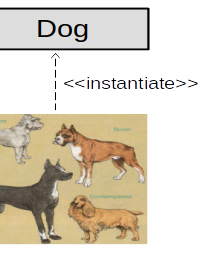
\includegraphics[width=0.5\linewidth]{img/instanziierung.png}}
    \caption{Visualization of the concept of instantiation in object-oriented programming}
    \label{fig:instantiation}
\end{figure}

Here a generated description of this picture (chatGPT):
\begin{quote}
This image is a visual metaphor for the \ac{oop} concept of instantiation.

Description:

- At the top of the image, there's a gray box labeled "Dog", which represents a class in OOP.

- Below it, there is a picture of different dog breeds (e.g., Boxer, Cocker Spaniel, etc.).

- A dashed arrow labeled <<instantiate>> points from the dog images to the class "Dog", indicating that these individual dogs are instances (objects) of the class.
\end{quote}

Simulation of electronic circuits is an important topic in technical electronics and technical informatics. Fig.~\ref{fig:rc} shows a screenshot of a circuit and a simulation result using the simulation tool LT-Spice.

\pagebreak

An AI-generated description of this figure can be improved if the context is given in the prompt: "explain this figure in the context of technical electronics"

\begin{figure}[ht]
    \centering
    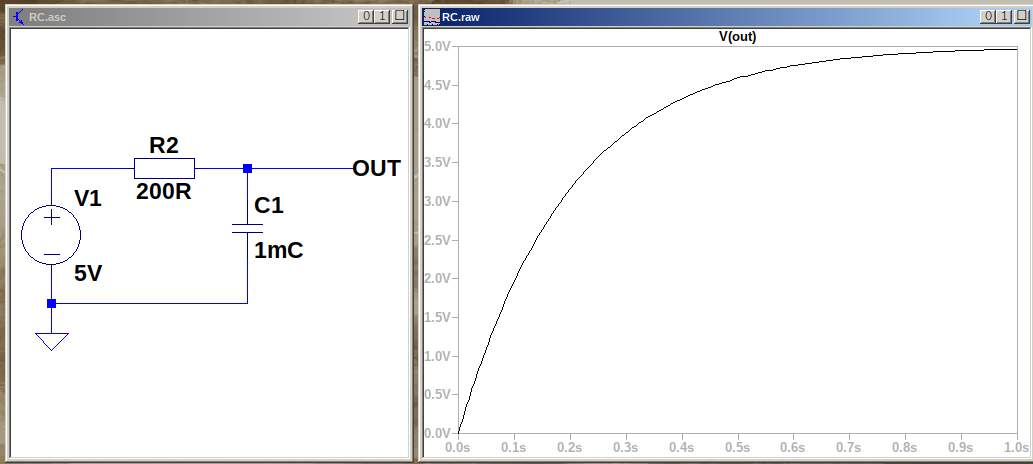
\includegraphics[width=0.9\linewidth]{img/RC.png}
    \caption{Screenshot of Circuit and Timeline Graph}
    \label{fig:rc}
\end{figure}


Answer from chatGPT:
\begin{quoted}
    

This figure illustrates the behavior of a simple RC (Resistor-Capacitor) charging circuit, commonly studied in technical electronics to understand transient response in linear time-invariant systems.

Left Side: Circuit Diagram

    The left side of the figure shows the schematic diagram of an RC circuit. It consists of:
\begin{itemize}
  \item A DC voltage source \( V_1 = 5\,\text{V} \)
  \item A resistor \( R_2 = 200\,\Omega \)
  \item A capacitor \( C_1 = 1\,\text{mF} \)
\end{itemize}

The resistor and capacitor are connected in series, and the voltage across the capacitor (marked as \texttt{OUT}) is observed over time. This configuration is typically used to study the charging process of a capacitor.

Right Side: Voltage-Time Plot

   The right side of the figure displays the simulation output: a voltage-time plot of \( V_{\text{out}} \), the voltage across the capacitor, from \( t = 0 \) to \( t = 1 \) second.

The voltage exhibits an exponential rise, which is characteristic of a capacitor charging through a resistor. The governing equation is:

\[
V(t) = V_{\text{source}} \cdot \left(1 - e^{-t/RC}\right)
\]

where:
\begin{itemize}
  \item \( V_{\text{source}} = 5\,\text{V} \)
  \item \( R = 200\,\Omega \)
  \item \( C = 1\,\text{mF} \)
  \item \( \tau = RC = 0.2\,\text{s} \) is the time constant
\end{itemize}

At approximately \( t = \tau \), the capacitor reaches about 63\% of its final value. The graph confirms that the capacitor voltage asymptotically approaches 5V, with the majority of charging occurring within the first second.

...

It serves as a fundamental demonstration of key concepts including time constants, exponential behavior, and transient analysis in electrical circuits.

\end{quoted}



\subsection*{Consequences}

% Benefits
\renewcommand{\labelenumi}{$+$}
\begin{enumerate}
\item The use of ‘alt text’ in HTML documents ensures that regulatory requirements for accessibility are better met. 

\item Generative AI can be used by authors to  create textual descriptions.

\item Generative AI tools can be integrated into your own applications. For example, a Python script can be used to add excellent "alt text" to entire folders full of images.


\item The generated explanation is not only helpful for blind and visually impaired people to gain access to the illustration. Sighted students can also benefit from this description.
\end{enumerate}

% Liabilities
\renewcommand{\labelenumi}{$-$}
\begin{enumerate}
\item Automatically generated descriptions should be checked by authors to ensure that the content is correct.
\end{enumerate}
 
\subsection*{Related Work}

The generation of explanatory text for graphics has been studied from both
automated and human-centered perspectives. Evaluations of automatic image
captioning systems show that while machine-generated descriptions can provide
basic accessibility, their quality often lacks accuracy and specificity,
highlighting the need for human editorial review
\cite{Leotta2023AutoCaptioning}. Complementary research on alternative text
creation documents the roles and processes through which authors, editors, and
reviewers collaboratively ensure reliable descriptions, emphasizing that
"alt text" production is a socio-technical practice rather than a purely
technical task \cite{Edwards2023AltTextProcess}. In addition, user studies with
blind and visually impaired participants underline that effective descriptions
must focus on data content, task relevance, and structural clarity rather than
only surface-level visual features \cite{Jung2021AltText}. Together, these
findings support our approach of combining automated captioning with
human-in-the-loop validation to ensure pedagogically useful and trustworthy
explanations of graphics.